\documentclass[../main.tex]{subfiles}
\graphicspath{{\subfix{../images/}}}

\begin{document}
 
\section{Εισαγωγή}

Στην εργασία αυτή μας ζητήθηκε να υλοποιήσουμε σε Verilog, ένα ψηφιακό σύστημα
αποστολέα-δέκτη, όπως παρουσιάζεται στο Σχήμα~\ref{fig:complete_system}. Η
επικοινωνία θα πραγματοποιείται με χρήση του πρωτοκόλλου UART. Ο αποστολέας θα
λαμβάνει από το περιβάλλον του τις ενδείξεις κάποιον αισθητήρων και ο δέκτης θα
εμφανίζει τις ενδείξεις που λαμβάνει σε μία οθόνη τεσσάρων LED 7-τμημάτων.

\begin{figure}[H]
  \begin{center}
    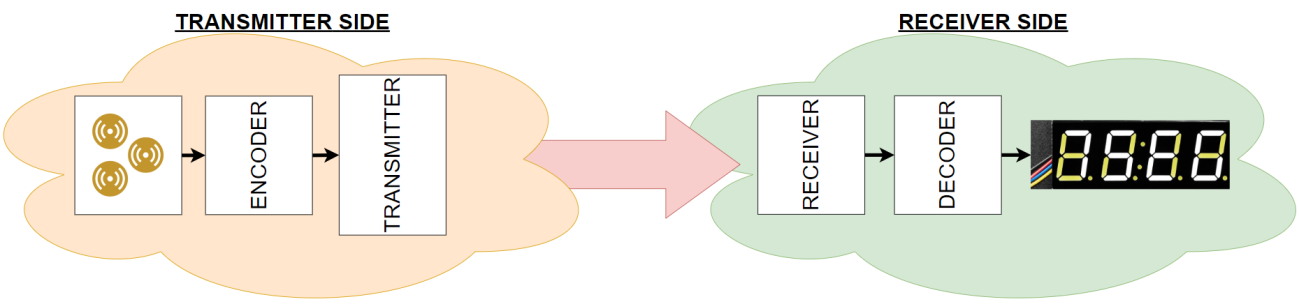
\includegraphics[width=0.95\textwidth]{images/complete_system.png}
  \end{center}
  \caption{Προεπισκόπηση της συνολικής υλοποίησης.}
  \label{fig:complete_system}
\end{figure}


\end{document}
